\documentclass[11pt]{article}

\usepackage{hyperref}
\usepackage{amsmath,amsfonts,amssymb}
\usepackage{mathpartir,mdframed,empheq}
\usepackage{mathtools}
\usepackage{ebproof}
\usepackage{braket} % Easy angle-bracket notation
\usepackage{parskip} %% Skips new paragraph indentation
\usepackage{bbm}
\usepackage{listings} % To typeset code
\lstset{
  basicstyle=\ttfamily,
  mathescape,
  breaklines=true
}
\usepackage{minted} %% Typeset code
\setminted{fontsize=\small}
\usepackage{bbold} %% For blackboard font
\usepackage{tikz} %% For drawing diagrams

\tikzset{every picture/.style={line width=0.75pt}} %set default line width to 0.75pt

%% Macro to facilitate the definition of variadic macros
%% from https://saswat.padhi.me/blog/2019-09_variadic-macros-in-latex/index.html
%% USAGE :: \VARIADIC {name} {start_sym} {mid_sym} {stop_sym}
\newcommand{\VARIADIC}[4]{%
  \expandafter\newcommand\csname Gobble#1Arg\endcsname[1]{%
    #3##1\csname Check#1Arg\endcsname%
  }%
  \expandafter\newcommand\csname Check#1Arg\endcsname{%
    \csname @ifnextchar\endcsname\bgroup{\csname Gobble#1Arg\endcsname}{#4}%
  }%
  \expandafter\newcommand\csname #1\endcsname[1]{%
    #2##1\csname Check#1Arg\endcsname%
  }%
}

\VARIADIC{Funapp} {} { \ } {} %% Function application by juxtaposition

\DeclarePairedDelimiter{\norm}{\lVert}{\rVert}

\newcommand\kw[1] {\textsf{#1}}
\newcommand\id[1] {\textsl{#1}}
\newcommand\latinphrase{\textit}

\NewDocumentCommand{\bI}{}{\mathbb{I}} %% Bold Interval I
\NewDocumentCommand{\ileft}{}{\id{i}_0} %% Interval i0
\NewDocumentCommand{\iright}{}{\id{i}_1} %% Interval i1
\NewDocumentCommand{\refl}{mg}{\IfValueTF{#2}{\kw{refl}_{#1} (#2)}{\kw{refl} (#1)}}

\NewDocumentCommand{\zpair}{}{\mathbb{Z}{\times}\mathbb{Z}{\ne}0}
\NewDocumentCommand{\equalq}{}{equal\mathbb{Q}}
\NewDocumentCommand{\zpairplus}{}{\mathbb{Z}{\times}\mathbb{Z}+}

\NewDocumentCommand{\oftype}{mmg}{\IfValueTF{#3}{#1\vdash#2:#3}{#1:#2}}
\NewDocumentCommand{\eqterm}{mmmg}{\IfValueTF{#4}{#1\vdash#2\equiv#3:#4}{#1\equiv#2:#3}}
\NewDocumentCommand{\eqtype}{mmg}{\IfValueTF{#3}{#1\vdash#2\equiv#3}{#1\equiv#2}}
\NewDocumentCommand{\ctx}{}{\Gamma}
\NewDocumentCommand{\earg}{mg}{\IfValueTF{#2}{#1:=#2}{\_:=#1}} %% Erasable argument

\newcommand\qed {\square}

\title{Quotient Types in Typer}
\author{James Tan \\ Université de Montréal \\ \href{mailto:james.juan.whei.tan@umontreal.ca}{james.juan.whei.tan@umontreal.ca}}

\date{September 11, 2023}

\begin{document}

\maketitle

\begin{abstract}
  TODO:Insert abstract
\end{abstract}

\tableofcontents

\section{Introduction}

\section{Cubical Equality}
\subsection{Interval type}
First, we provide the typical definition of the \id{Interval} type, subsequently we present our alternative formulation of the \id{Interval} type and show that it is equivalent to the traditional definition.

\begin{prooftree*}
   \infer0{\oftype{\ctx}{\bI}{Type}}
\end{prooftree*}

\begin{prooftree*}
   \infer0{\oftype{\ctx}{i_{0}}{\bI}}
\end{prooftree*}

\begin{prooftree*}
   \infer0{\oftype{\ctx}{i_{1}}{\bI}}
\end{prooftree*}

\begin{prooftree*}
   \infer0{\oftype{\ctx}{seg}{\eqtype{i_0}{i_1}}}
\end{prooftree*}

We postulate the existence of the unit interval, along with the ends of the interval \id{$i_0$} and \id{$i_1$}. We also have \id{seg} which is a witness of a continuous path between \id{$i_0$} and \id{$i_1$}.

Elimination of $\bI$ is similar to that of \id{Booleans} the only difference is that a proof must be provided to prove that $\eqtype{i_0}{i_1}$ is respected. The recursion principle of $\bI$ can thus be stated as follows:

\begin{prooftree*}
   \hypo{\oftype{\ctx}{A}{Type}}
   \hypo{\oftype{\ctx}{M}{A}}
   \hypo{\oftype{\ctx}{N}{A}}
   \hypo{\oftype{\ctx}{P}{\eqtype{M}{N}}}
   \infer4{\oftype{\ctx, \oftype{i}{\bI}}{rec_{\bI} (\_.\ A, M, N, P, i)}{A}}
\end{prooftree*}

The recursion principle computes as follows:

\begin{align*}
  & rec_{\bI}(\_ . A, M, N, P, \ileft) = M \\
  & rec_{\bI}(\_ . A, M, N, P, \iright) = N \\
  & \kw{cong}_{rec_{\bI}(\_ . A, M, N, P)}(\id{seg}) = P
\end{align*}

We can expect the first two equations to hold definitionally. If we imagine that the first two computation rules were defined via pattern-matching, it would make sense for the equations to hold definitionally. However, more often than not, the third equation only holds propositionally, as is the case when such a type is defined in other type systems, e.g. Agda. (TODO:\ Might have to improve the phrasing, the entire thing might not be relevant at all, idk we'll see)

TODO:\ The proof below requires depelim of Interval?

\subsection{Motivation}
We show that a function out of the interval into some type \id{A} is equivalent to a path between two terms of type \id{A}, in other words, we show the following

\begin{align*}
  & \bI \rightarrow A \simeq \Sigma_{\oftype{x}{A}} . \Sigma_{\oftype{y}{A}} . \eqtype{x}{y}
\end{align*}

We take equivalence to mean what it means in the HoTT book (TODO:\ rephrase this). To prove the above, we define a function \id{f} and its inverse \id{g} as such:

\begin{align*}
  & f : (\bI \rightarrow A) \rightarrow \Sigma_{\oftype{x}{A}} . \Sigma_{\oftype{y}{A}} . \eqtype{x}{y} \\
  & f(h) := \braket{\id{h}(\ileft), \braket{\id{h}(\iright), \kw{cong}_{\id{h}}(\id{seg})}} \\ \\
  & g : \Sigma_{\oftype{x}{A}} . \Sigma_{\oftype{y}{A}} . (\eqtype{x}{y}) \rightarrow  (\bI \rightarrow A) \\
  & g \braket{x, \braket{y, p}} := \lambda \id{i} . rec_{\bI}(\_ . \id{A}, \id{x}, \id{y}, \id{p}, \id{i})
\end{align*}

Now, we need to prove that \id{g} is both the left and right inverse of \id{f}.

TODO:\ Add proof of $\kw{cong}_2$ and $\Sigma$ path characterisation in the appendix or something (sketch is in Interval.lagda.md)

\begin{align*}
  & \id{$\alpha$-helper} : (\oftype{h}{\bI \rightarrow A}) \rightarrow (\oftype{i}{Interval}) \rightarrow \eqtype{(g (f \ h)) \ i}{h \ i} \\
  & \id{$\alpha$-helper} (h , i) = rec_{\bI}(i . \ \eqtype{(g (f \ h)) \ i}{h \ i}, \ \refl{h(\ileft)}, \ \refl{h(\iright)}, \ \kw{cong}_{\lambda i . \refl{h(i)}}(\id{seg}), \ i) \\
  & \alpha : (\oftype{h}{\bI \rightarrow A}) \rightarrow \eqtype{g(f(h))}{h} \\
  & \alpha(h) =  \kw{funExt} (\id{$\alpha$-helper} (h)) \\ \\
  & \beta :  (\oftype{e}{\Sigma_{\oftype{x}{A}} . \Sigma_{\oftype{y}{A}} . \eqtype{x}{y}}) \rightarrow f(g(e)) = e \\
  & \beta(e) =  \refl{\Sigma_{\oftype{x}{A}} . \Sigma_{\oftype{y}{A}} . \eqtype{x}{y}}{e}
\end{align*}

For the sake of simplifying the proof of $\beta$, we assume the $\eta$-rule for dependent pairs. And with that, the proof is complete.

\subsection{Justification}
We have established that the equality type (also known as the identity type) is equivalent to a function out of the interval. We have also illustrated that such a function is expected to be constant on the unit interval. This `condition' is enforced by virtue of the fact that $\id{Interval}$ is defined as a higher inductive type with an identification of its two `points' (TODO:\ wording?). An alternate way of enforcing this is to use erasable functions out of a $\mathbbm{2}$-type. In other words, we can first define the $\id{Interval}$ type as a normal algebraic data type.

TODO:\ Define/explain erasable functions

\begin{minted}[escapeinside=@@,mathescape=true]{haskell}
type I
  | @$i_0$@
  | @$i_1$@
\end{minted}

And then define a function with the following type:

\begin{minted}[escapeinside=@@,mathescape=true]{haskell}
h : I @$\Rrightarrow$@ A
\end{minted}

Then, it is vacuously true that $\eqtype{h(i_0)}{h(i_1)}$. With that, we are able to postulate that

\begin{align*}
  & \bI \Rrightarrow A \simeq \Sigma_{\oftype{x}{A}} . \Sigma_{\oftype{y}{A}} . \eqtype{x}{y}
\end{align*}

The above shall be the basis of our new definition of identity types.

\subsection{Elimination of the Interval type}
TODO:\ Mention transp

\subsection{Manipulation of the Interval type}
TODO:\ Mention operators like $\!$, $\wedge$ and $\vee$.

\subsection{Identity type}

\subsubsection{Heterogenous equality}
With the above definition of $\bI$, we are now ready to introduce the notion of heterogenous equality. Such an equality type allows us to identify two terms that are not necessarily of the same type. The heterogenous equality type has the following type signature\footnote{Although not mentioned explicitly, functions involving the identity type are universe polymorphic in their arguments and return type.} and is implemented axiomatically.

\begin{minted}[escapeinside=@@,mathescape=true]{haskell}
Heq : ?x @$\rightarrow$@ ?y @$\rightarrow$@ Type
\end{minted}

The introduction rule of the above type leverages the fact that erasable functions out of the interval are equivalent to identity types.

%% Heq_eq : (l : TypeLevel) ≡> (t : I ≡> Type_ l) ≡> (f : (i : I) ≡> t (_ := i))
%%           ≡> Heq (f (_ := i0)) (f (_ := i1))

\begin{minted}[escapeinside=@@,mathescape=true]{haskell}
Heq_eq : (t : I @$\Rrightarrow$@ Type)
         @$\Rrightarrow$@ (f : (i : I) @$\Rrightarrow$@ t (_ := i))
         @$\Rrightarrow$@ Heq (f (_ := i0)) (f (_ := i1))
\end{minted}

The elimination of equality types is trivial, it merely returns a function out of the interval that represents the underlying equality.

%% Heq_uneq : (l : TypeLevel) ≡> (t : I ≡> Type_ l)
%%                     ≡> (x : t (_ := i0)) => (y : t (_ := i1))
%%                     => (p : Heq x y) ≡> (i : I) ≡> t (_ := i)
\begin{minted}[escapeinside=@@,mathescape=true]{haskell}
Heq_uneq : (t : I @$\Rrightarrow$@ Type)
           @$\Rrightarrow$@ (x : t (_ := i0)) @$\Rightarrow$@ (y : t (_ := i1))
           @$\Rightarrow$@ (p : Heq x y) @$\Rrightarrow$@ (i : I) @$\Rrightarrow$@ t (_ := i)
\end{minted}

The composition of $\id{Heq\_uneq}$ and  $\id{Heq\_eq}$ (modulo the implicit arguments) is equal to the identity function.

\subsubsection{Homogenous equality}
Homogenous equality is by far the more typical notion of equality. We are able to define it as a special case of heterogenous equality where the two terms $\id{x}$ and $\id{y}$ in $\Funapp{\id{Heq}}{\id{x}}{\id{y}}$ are of the same type.

%% TODO: Fix the alignment
%% Eq_uneq : (l : TypeLevel) ≡> (t : Type_ l)
%%           ≡> (x : t) => (y : t)
%%           => (p : Eq x y) ≡> (i : I) ≡> t
%% Eq_uneq = lambda _ ≡> lambda t ≡>
%%             lambda _ => lambda _ =>
%%               lambda p ≡> lambda i ≡>
%%                 Heq_uneq (t := lambda _ ≡> t) (p := p) (i := i)
\begin{minted}[escapeinside=@@,mathescape=true]{haskell}
Eq : (t : Type) @$\Rrightarrow$@ t @$\rightarrow$@ t @$\rightarrow$@ Type
Eq x y = Heq x y

Eq_eq : (t : Type) @$\Rrightarrow$@ (f : I @$\Rrightarrow$@ t)
        @$\Rrightarrow$@ Eq (t := t) (f (_ := @$\ileft$@)) (f (_ := @$\iright$@))
Eq_eq t f = Heq_eq (t := @$\lambda$@ _ @$\Rrightarrow$@ t) (f := f)

Eq_uneq : (t : Type) @$\Rrightarrow$@ (x : t) @$\Rightarrow$@ (y : t) @$\Rightarrow$@ (p : Eq x y)
          @$\Rrightarrow$@ (i : I) @$\Rrightarrow$@ t
Eq_uneq p i = Heq_uneq (t := @$\lambda$@ _ @$\Rrightarrow$@ t) (p := p) (i := i)
\end{minted}

\subsection{Reduction rules}

\begin{prooftree*}
   \infer0[UNEQ-LEFT]{\Funapp{\id{Heq\_uneq}}{\id{x}}{\id{y}}{\id{p}}{\ileft}
                     \rightsquigarrow \id{x}}
\end{prooftree*}

\begin{prooftree*}
   \infer0[UNEQ-RIGHT]{\Funapp{\id{Heq\_uneq}}{\id{x}}{\id{y}}{\id{p}}{\iright}
                       \rightsquigarrow \id{y}}
\end{prooftree*}

\subsection{Examples}
Common properties of the equality type remain true, some of them are easier to prove than with a traditional equality type.

\subsubsection*{Reflexivity}
A reflexive equality is the most trivial equality that we are able to construct, and indeed, it is the one that we are able to construct with an erasable function out of $\bI$ given that such a function is necessarily a constant function.

%% Eq_refl : (l : TypeLevel) ≡> (t : Type_ l)
%%            ≡> (x : t) ≡> Eq x x
%% Eq_refl = lambda _ ≡> lambda _ ≡> lambda x ≡>
%%             Eq_eq (f := lambda _ ≡> x)
\begin{minted}[escapeinside=||,mathescape=true]{haskell}
Eq_refl : (x : ?t) |$\Rrightarrow$| Eq x x
Eq_refl x = Eq_eq (f := |$\lambda$| _ |$\Rrightarrow$| x)
\end{minted}

\subsubsection*{Commutativity}
This is the first of many properties that can be proved in an elegant manner by virtue of defining the equality type based on functions out of the interval. This property has many names, such as the commutativity of equality, the symmetry of equality, or the inversion of a path. Consider an equality between $\id{x}$ and $\id{y}$, we can think of the two terms as points, the equality itself can then be thought of as a continuous path between the two points. We think of the path as a directed path from $\id{x}$ to $\id{y}$. The commutativity of equality basically means that we are able to construct a path that goes in the opposite direction, in other words, we are able to invert the path. This is the intuition behind the following proof.

%% Eq_comm : (x : ?t) ≡> (y : ?t) ≡> Eq x y -> Eq y x
%% Eq_comm p = Eq_eq (f := lambda i ≡> Eq_uneq (p := p) (i := I_not i))
\begin{minted}[escapeinside=||,mathescape=true]{haskell}
Eq_comm : (x y : ?t) |$\Rrightarrow$| Eq x y |$\rightarrow$| Eq y x
Eq_comm x y = Eq_eq (f := |$\lambda$| i |$\Rrightarrow$| Eq_uneq (p := p) (i := !i))
\end{minted}

\subsubsection*{Functional extensionality}
The notion of functional extensionality implies that pointwise-equal functions are indeed equal. By postulating the existence of the $\id{Interval}$ type along with an equality type that's based on it, functional extensionality can be derived trivially as is illustrated by the below proof.

\begin{minted}[escapeinside=||,mathescape=true]{haskell}
Eq_funExt : (f : (? |$\rightarrow$| ?)) |$\Rightarrow$| (g : (? |$\rightarrow$| ?))
            |$\Rightarrow$| (p : (x : ?) |$\rightarrow$| Eq (f x) (g x)) |$\rightarrow$| Eq f g
Eq_funExt p = Eq_eq (f := |$\lambda$| i |$\Rrightarrow$| |$\lambda$| x |$\rightarrow$|
                                   Eq_uneq (p := p x) (i := i))
\end{minted}

We note that the above proof makes use of the $\eta$-equivalence of functions, i.e. $\lambda \id{x} \rightarrow \Funapp{\id{f}}{\id{x}} \equiv \id{f}$. Another thing that is worth noting is that we interpret erasable functions out of $\bI$ themselves as an equality type, i.e.\ if we do without the $\id{Eq\_eq}$ constructor, and if we we think of $\id{Eq\_uneq}$ as the direct application of an expression of type $\bI$  to such a function, we obtain the following interpretation of $\id{Eq\_funExt}$.

\begin{minted}[escapeinside=||,mathescape=true]{haskell}
Eq_funExt : (f : (? |$\rightarrow$| ?)) |$\Rightarrow$| (g : (? |$\rightarrow$| ?))
            |$\Rightarrow$| (p : (x : ?) |$\rightarrow$| Eq (f x) (g x)) |$\rightarrow$| Eq f g
Eq_funExt p i x = p x i
\end{minted}

In this case, it becomes clear that $\id{Eq\_funExt}$ is a trivial function that does no more than swap the order of its two arguments. This is observed in several recent proof assistants that implement cubical type theory, such as Cubical Agda, coolTT and redTT.\@

TODO:\ Decide if the below is worth mentioning in some way \\
Note: funExt is required to prove quotient effectiveness, though we will see that the existence of $\id{Quotient}$ implies $\id{funExt}$.

%% FIXME: Should this come before the section on funext? probably
\subsubsection*{Congruence of equality}
This is a another typical property of equality that is proven with a `cubical' equality.

%% Eq_cong : (x : ?A) => (y : ?A) =>
%%           (f : ?A -> ?) -> (p : Eq x y)
%%           -> Eq (f x) (f y)
%% Eq_cong = lambda f -> lambda p ->
%%             Eq_eq (f := lambda i ≡> f (Eq_uneq (p := p) (i := i)))
\begin{minted}[escapeinside=||,mathescape=true]{haskell}
Eq_cong : (x y : ?A) |$\Rightarrow$| (f : (?A |$\rightarrow$| ?)) |$\rightarrow$| (p : Eq x y)
          |$\rightarrow$| Eq (f x) (f y)
Eq_cong f p = Eq_eq (f := |$\lambda$| i |$\Rrightarrow$| f (Eq_uneq (p := p) (i := i)))
\end{minted}


Like before, with a slight change of perspective, we see that the congruence of equality merely involves applying the function $\id{f}$ `inside' the equality.

\begin{minted}[escapeinside=||,mathescape=true]{haskell}
Eq_cong : (x y : ?A) |$\Rightarrow$| (f : (?A |$\rightarrow$| ?)) |$\rightarrow$| (p : Eq x y)
          |$\rightarrow$| Eq (f x) (f y)
Eq_cong f p i = f (p i)
\end{minted}

\subsubsection*{Transport}
The transport operation (also known as {\id{cast}}) allows us to transport properties that are true for some type $\id{A}$ to another type $\id{B}$ if we have a proof that $\eqtype{\id{A}}{\id{B}}$.

%% Eq_cast : (x : ?) ≡> (y : ?) ≡> (p : Eq x y) ≡> (f : ? -> ?)
%%             ≡> f x -> f y
%% Eq_cast = lambda _ ≡> lambda _ ≡> %% Two level variables
%%            lambda A ≡> %% Type of x and y
%%            lambda x ≡> lambda y ≡>
%%            lambda p ≡> lambda f ≡>
%%              lambda fx ->
%%                 I_transp (A := lambda i ≡> f (Heq_uneq
%%                                               (t := lambda _ ≡> A)
%%                                               (p := p) (i := i)))
%%                          (r := i0) fx
%%

\begin{minted}[escapeinside=||,mathescape=true]{haskell}
Eq_cast : (x y : ?A) |$\Rrightarrow$| (p : Eq x y) |$\Rrightarrow$| (f : (? |$\rightarrow$| ?)) |$\Rrightarrow$| f x
          |$\rightarrow$| f y
Eq_cast A x y p f fx =
  I_transp (A := |$\lambda$| t |$\Rrightarrow$| f (Eq_uneq (t := t) (p := p) (i := i)))
           (r := |$\ileft$|) fx
\end{minted}

Here, we make use of the built-in function $\id{I\_transp}$ by passing it the argument $\earg{\id{r}}{\ileft}$, intending it to behave as a transport function. In other words, by passing it something of type $\Funapp{\id{f}}{\id{x}}$, it returns something of type $\Funapp{\id{f}}{\id{y}}$, which is precisely what the transport/cast function is meant to do.

The $\id{I\_transp}$ function that looks slightly strange at first sight allows us to prove a certain property of the transport operation. Transporting across a reflexive path should be equivalent to a no-op, as is illustrated in the following proof.

\begin{minted}[escapeinside=||,mathescape=true]{haskell}
Eq_cast_refl : (A : Type) |$\Rrightarrow$| (x : A)
               |$\rightarrow$| Eq (Eq_cast (p := Eq_refl (x := x))
                              (f := |$\lambda$| _ |$\rightarrow$| A) x)
                     x
Eq_cast_refl A x = Eq_eq (f := |$\lambda$| i |$\Rrightarrow$|
                            I_transp (A := |$\lambda$| _ |$\Rrightarrow$| A) (r := i) x)
\end{minted}

\subsubsection*{Transitivity}\label{subsubsection:eqtransitivity}
Continuing our analogy of equality proofs as paths, the transitivity property allows us to concatenate two paths. We join the right endpoint of the first path with the left endpoint of the second path, producing a new path. The proof of this theorem is as follows:

\begin{minted}[escapeinside=||,mathescape=true]{haskell}
Eq_trans : (x y z: ?t) |$\Rrightarrow$| Eq x y |$\rightarrow$| Eq y z |$\rightarrow$| Eq x z
Eq_trans x y z x=y y=z = Eq_cast (p := y=z)
                                 (f := |$\lambda$| x' |$\rightarrow$| Eq x x')
                                 x=y
\end{minted}

\subsection{Limitations}
We don't have primitives such as $hcomp$, what does this imply? Is there a certain class of proofs we are unable to construct? Or do we just suffer from some amount of inconvenience?


\section{Quotient Rules}
\subsection{Typing}
We present the $\id{Quotient}$ primitives along with their typing rules.

\begin{prooftree*}
   \hypo{\oftype{\ctx}{\id{A}}{\kw{Type}}}
   \hypo{\oftype{\ctx}{\id{R}}{\id{A} \rightarrow \id{A} \rightarrow \kw{Type}}}
   \infer2[\kw{QUOT-FORMATION}]{\oftype{\ctx}{\Funapp{\id{Quotient}}{\id{A}}{\id{R}}}
                                             {\kw{Type}}}
\end{prooftree*}

\begin{prooftree*}
   \hypo{\oftype{\ctx}{\id{a}}{\id{A}}}
   \hypo{\oftype{\ctx}{\Funapp{\id{Quotient}}{\id{A}}{\id{R}}}
                      {\kw{Type}}}
   \infer2[\kw{QUOT-INTRO-IN}]{\oftype{\ctx}{\Funapp{\id{Quotient\_in}}{\id{A}}{\id{R}}{\id{a}}}
                                         {\Funapp{\id{Quotient}}{\id{A}}{\id{R}}}}
\end{prooftree*}

\begin{prooftree*}
   \hypo{\oftype{\ctx}{\id{a}_1}{\id{A}}}
   \hypo{\oftype{\ctx}{\id{a}_2}{\id{A}}}
   \hypo{\oftype{\ctx}{\id{r}}{\Funapp{\id{R}}{\id{a}_1}}{\id{a}_2}}
   \infer3[\kw{QUOT-INTRO-EQ}]{\oftype{\ctx}{\Funapp{\id{Quotient\_eq}}{\id{A}}{\id{R}}{\id{a}_1}{\id{a}_2}{\id{r}}}
                                      {\Funapp{\id{Eq}}{(\Funapp{\id{Quotient\_in}}{\id{A}}{\id{R}}{\id{a}_1})}
                                                       {(\Funapp{\id{Quotient\_in}}{\id{A}}{\id{R}}{\id{a}_2})}}}
\end{prooftree*}

\begin{prooftree*}
   \hypo{\oftype{\ctx}{\id{P}}{\Funapp{\id{Quotient}}{\id{A}}{\id{R}} \rightarrow \kw{Type}}}
   \hypo{\oftype{\ctx}{\id{q}}{\Funapp{\id{Quotient}}{\id{A}}{\id{R}}}}
   \infer[no rule]2{\oftype{\ctx}{\id{f}}{(\oftype{\id{a}}{\id{A}})
                                    \rightarrow \Funapp{\id{P}}{(\Funapp{\id{Quotient\_in}}{\id{A}}{\id{R}}{\id{a}}})}}
   \infer[no rule]1{\oftype{\ctx}{\id{h}}{(\oftype{\id{a}_1 \ \id{a}_2}{\id{A}})
                                          \rightarrow \Funapp{\id{R}}{\id{a}_1}{\id{a}_2}}
                                          \rightarrow \Funapp{\id{Heq}}{(\Funapp{\id{f}}{\id{a}_1})}
                                                                       {(\Funapp{\id{f}}{\id{a}_2})}}
   \infer1[\kw{QUOT-ELIM}]{\oftype{\ctx}{\Funapp{\id{Quotient\_elim}}{\id{A}}{\id{R}}{\id{f}}{\id{h}}{\id{q}}}
                                        {\Funapp{\id{P}}{\id{q}}}}
\end{prooftree*}


\subsection{Reductions}
We present the computation rule for the elimination of quotients.

\begin{prooftree*}
   \hypo{\id{q} \rightsquigarrow \Funapp{\id{Quotient\_in}}{\id{A}}{\id{R}}{\id{a}}}
   \infer1[]{\Funapp{\id{Quotient\_elim}}{\id{A}}{\id{R}}{\id{f}}{\id{h}}{\id{q}}
             \rightsquigarrow \Funapp{\id{f}}{\id{a}}}
\end{prooftree*}

We see that during $\id{Quotient}$ elimination, the proof that the eliminator function respects the $\id{Quotient}$ is ignored. Instead, the function is applied directly to the underlying element of the base type.

\section{Implementation}
In this chapter, we describe how we added quotient types to Typer. Next, we describe the library that we provide to facilitate the usage of quotient types in the development of Typer programs and proofs.

\subsection{Axioms}
Quotient types are introduced in Typer in axiomatic manner, in other words, we postulate the existence of quotient types and define their behaviour axiomatically.

\subsubsection*{Formation}
The existence of the $\id{Quotient}$ type is postulated as follows

\begin{minted}[escapeinside=||,mathescape=true]{haskell}
Quotient : (A : Type) |$\rightarrow$| (R : A |$\rightarrow$| A |$\rightarrow$| Type) |$\rightarrow$| Type
\end{minted}

\subsubsection*{Introduction}
Two axioms are added, corresponding to the two introduction rules of $\id{Quotient}$.

\begin{minted}[escapeinside=||,mathescape=true]{haskell}
Quotient_in : (A : Type) |$\Rrightarrow$| (R : A |$\rightarrow$| A |$\rightarrow$| Type) |$\Rrightarrow$| A |$\rightarrow$| Quotient A R
Quotient_eq : (A : Type) |$\Rrightarrow$| (R A |$\rightarrow$| A |$\rightarrow$| Type)  |$\Rrightarrow$| (a a' : A) |$\Rrightarrow$| R a a'
              |$\rightarrow$| Eq (Quotient_in (R := R) a) (Quotient_in (R := R) a')
\end{minted}

\subsubsection*{Elimination}

\begin{minted}[escapeinside=||,mathescape=true]{haskell}
Quotient_elim : (A : Type) |$\Rrightarrow$| (R : A |$\rightarrow$| A |$\rightarrow$| Type)
                |$\Rrightarrow$| (P : Quotient A R |$\rightarrow$| Type})
                |$\Rrightarrow$| ((a : A) |$\rightarrow$| P (Quotient_in a))
                |$\rightarrow$| ((a a' : A) |$\rightarrow$| R a a' |$\rightarrow$| Heq (f a) (f a')
                |$\Rrightarrow$| (q : Quotient A R) |$\rightarrow$| P q
\end{minted}

\subsection{Syntaxique sugar}
TODO: Add after things get figured out

\section{Quotient Effectiveness}
This only works for relations that are propositions and equivalence relations (i.e.\ reflexive, symmetric and transitive).
\subsection{Propositional Extensionality}
We provide a `weaker' (or alternative? which is it?) version of propositional extensionality. With this, we prove (a weaker version) quotient effectiveness.

\subsubsection{Representation of propositions}
TODO: Describe the $Erased$ type and a proof that $\id{isProp (Erased A)}$.

Intuitively speaking, propositions are a type that contain no intrinsic data, it is their mere existence that counts. This is precisely the notion of proof irrelevance. In Typer, this notion is represented via erasability. We introduce a built-in data type that captures this idea.

\begin{minted}{haskell}
type Erased (T : Type)
  | erased (t ::: T)
\end{minted}

By ensuring that the witness $\id{t}$ of the type $\id{T}$ is erasable, this provides us with a guarantee that during elimination, the witness $\id{t}$ can only be used in an erasable, i.e.\ proof irrelevant manner.

To convince ourselves that this type does indeed capture the essence of a proposition, we provide a proof of $\Funapp{\id{isProp}}{(\Funapp{\id{Erased}}{?\id{T}})}$. We state the definition of $\id{isProp}$:

\begin{minted}[escapeinside=||,mathescape=true]{haskell}
isProp : (T : Type) |$\rightarrow$| Type
isProp T = (x y : T) |$\rightarrow$| Eq x y
\end{minted}

We now the present the proof in the form of Typer code.

\begin{minted}[escapeinside=@@,mathescape=true]{haskell}
erasedIsProp : (T : Type) @$\Rrightarrow$@ isProp (Erased T)
erasedIsProp t1 t2 =
  case t1
    | erased (_ := e1) @$\Rightarrow$@
        let
          p1 = ##DeBruijn 0 : Eq (erased (t := e1)) t1
        in
          case t2
            | erased (_ := e2) @$\Rightarrow$@
                let
                  p2 = ##DeBruijn 0 : Eq (erased (t := e2)) t2
                in
                  Eq_trans (Eq_comm p1) p2
\end{minted}

Typer does not offer the direct specialisation of $\kw{case}$ targets in branches. In other words, in the first case branch, we do not have a definitional equality between $\id{t1}$ and $\Funapp{\id{erased}}{(\earg{\_}{\id{e1}})}$. Instead, an equality proof between them is injected into the context, which can be accessed as the variable at deBruijn index 0. Now that we have the two equality proofs, in order to concatenate them \footnote{By considering equalities as path, the application of the transitivity property of equality is conceptually similar to concatenating two paths.}, we require $\Funapp{\id{erased}}{(\earg{\_}{\id{e1}})}$ and $\Funapp{\id{erased}}{(\earg{\_}{\id{e2}})}$ to be equal. A priori, the two terms are not equal as $\id{e1}$ and $\id{e2}$ are completely arbitrary. However, Typer ignores erasable terms when checking the convertibility of terms, this is a property that was proven to be sound in ??? (TODO: Cite ICC paper). This allows the concatenation to succeed and thus concludes the proof.

\subsubsection{Axiom}
Propositional extensionality essentially means that if two propositions that are logically equivalent, i.e.\ each proposition implies the other, then we can say that they are equal. And precisely because we are postulating a new equality constructor, we have to be very careful that the resulting equality proof is indeed proof irrelevant. In other words, we need this equality proof to not have any runtime relevance. This is principally because we insist that the transport operation to be a no-op during runtime. This is the motivation behind our choice to use the $\id{Erased}$ type to represent propositions, as it is a guarantee that such a type carries no useful runtime information. This implies that a transport operation from one $\id{Erased}$ type to another is simply a no-op.

In a setting with univalence, propositional extensionality is simply a theorem that may be proven (TODO:\ Maybe cite something here). This is a result that is immediate as an equivalence between logically equivalent propositions is trivial. In the setting of Typer however, propositional extensionality is implemented as an axiom with the following type signature:

\begin{minted}[escapeinside=@@,mathescape=true]{haskell}
propExt : (A : Type) @$\Rrightarrow$@ (B : Type) @$\Rrightarrow$@ (Erased A @$\rightarrow$@ Erased B)
           @$\rightarrow$@ (Erased B @$\rightarrow$@ Erased A) @$\rightarrow$@ Eq (Erased A) (Erased B)
\end{minted}

The above is a weaker notion of propositional extensionality compared to what is proposed in Cubical Agda, which has the following type signature:

\begin{minted}[escapeinside=@@,mathescape=true]{Agda}
propExt : {A B : Type} @$\rightarrow$@ isProp A @$\rightarrow$@ isProp B @$\rightarrow$@ (A @$\rightarrow$@ B)
          @$\rightarrow$@ (B @$\rightarrow$@ A) @$\rightarrow$@ A @$\equiv$@ B
\end{minted}

However, this produces an equality proof that is not proof irrelevant, which we illustrate with a simple example. We define two instances of the unit type which are trivially `logically equivalent'.

\begin{minted}[escapeinside=@@,mathescape=true]{Agda}
data Unit1 : Type where
  unit1 : Unit1

data Unit2 : Type where
  unit2 : Unit2
\end{minted}

$\Funapp{\kw{isProp}}{\id{Unit1}}$ and $\Funapp{\kw{isProp}}{\id{Unit2}}$ are trivially true, as is the case for all $\mathbb{1}$ types. $\id{Unit1} \rightarrow \id{Unit2}$ and $\id{Unit2} \rightarrow \id{Unit1}$ are also inhabited. Propositional extensionality thus gives us a proof of $\id{Unit1} \equiv \id{Unit2}$. This implies that we should be able to use said proof to transport $\id{unit1}$ to $\id{unit2}$, but since the two terms do not have the same runtime value, this simply cannot be a no-op.

Another worthy comparison to make is with Lean, which has a $\kw{Prop}$ sort. Terms of this sort are not autorised to be used in a proof relevant manner. Its version of propositional extensionality has the following form:

\begin{minted}[escapeinside=@@,mathescape=true]{lean}
axiom propext {a b : Prop} : (a @$\leftrightarrow$@ b) @$\rightarrow$@ a = b
\end{minted}

This is similar to what we have in Typer, except that proof irrelevance is enforced in a different manner.

\subsection{Equivalence relation}
TODO: Explanation of relations should probably go elsewhere

First, we state what we mean when we say `relation' to set the stage for the subsequent discussion. For our purposes, we conider binary relations, which are type formers that take two arguments of some type $\kw{A}$. Assuming that we call the relation $\kw{R}$ and its two arguments $\id{a}$ and $\id{a}'$ respectively, inhabitants of the type $\Funapp{\kw{R}}{\id{a}}{\id{a}'}$ are witnesses of this binary relation. The type signature of a binary relation has the below form:

\begin{minted}[escapeinside=||,mathescape=true]{haskell}
R : (A : Type) |$\Rrightarrow$| (a : A) |$\rightarrow$| (a' : A) |$\rightarrow$| Type
\end{minted}

For a quotient to be effective, its underlying relation has to be an equivalence relation, we shall use this property in the proof in the subsequent section. Recall that an equivalence relation implies that the relation is reflexive, symmetric and transitive. For it to be reflexive, it needs to be the case that given an arbitrary $\oftype{\id{a}}{\kw{A}}$, $\Funapp{\kw{R}}{\id{a}}{\id{a}}$ must be trivially inhabited. The symmetry of the relation implies that if we are given an arbitrary witness of $\Funapp{\kw{R}}{\id{a}}{\id{a}'}$, we need to be able to transform that into an inhabitant of $\Funapp{\kw{R}}{\id{a}'}{\id{a}}$. The relation is transitive if we are able to transform witnesses of $\Funapp{\kw{R}}{\id{a}}{\id{b}}$ and $\Funapp{\kw{R}}{\id{b}}{\id{c}}$ into witnesses of $\Funapp{\kw{R}}{\id{a}}{\id{c}}$. \footnote{The equality type fulfills these criteria and is an equivalence relation.}

In the built-in library, we define the following type as a witness that a certain relation is indeed an equivalence relation.

\begin{minted}{haskell}
type isEquivRel (A : Type) (R : A -> A -> Type) : Type
  | equivRel (isRefl : (a : A) -> R a a)
             (isSym : (a : A) -> (b : A) -> R a b -> R b a)
             (isTrans : (a : A) -> (b : A) -> (c : A)
                         -> R a b -> R b c -> R a c)
\end{minted}

\subsection{Proof}
Given two arbitrary elements $\id{a}$ and $\id{a}'$ of a base type $\kw{A}$, a quotient is said to be effective if given a proof that the injection of $\id{a}$ and $\id{a}'$ into the quotient are equal, then it must be the case that $\Funapp{\kw{R}}{\id{a}}{\id{a}'}$ is true, i.e.\ we are able to find an inhabitant of it. A sufficient condition for a quotient to be effective is that the underlying relation must be both a proposition and an equivalence relation.


For an arbitrary binary relation $\kw{R}$, we can define the following:

\begin{minted}[escapeinside=||,mathescape=true]{haskell}
ErasedR : (A : Type) |$\Rrightarrow$| (A |$\rightarrow$| A |$\rightarrow$| Type) |$\rightarrow$| A |$\rightarrow$| A |$\rightarrow$| Type
ErasedR R a b = Erased (R a b)
\end{minted}

Now, we state the proof of the effectiveness of quotients in the form of Typer code

\begin{minted}[escapeinside=||,mathescape=true]{haskell}
effective : (A : Type) |$\Rrightarrow$| (R : A |$\rightarrow$| A |$\rightarrow$| Type)
            |$\rightarrow$| isEquivRel A (ErasedR R) |$\rightarrow$| (a : A) |$\rightarrow$| (b : A)
            |$\rightarrow$| Eq (Quotient_in (R := ErasedR R) a)
                  (Quotient_in (R := ErasedR R) b)
            |$\rightarrow$| ErasedR R a b
effective = lambda A |$\Rrightarrow$| lambda R equiv a b eq |$\rightarrow$|
  let
    helper : Quotient A (ErasedR R) -> Type
    helper x =
      Quotient_rec
        (R := ErasedR R)
        (lambda c |$\rightarrow$| ErasedR R a c)
        (p := lambda c d cd |$\rightarrow$|
          let
            ac->ad : Erased (R a c) |$\rightarrow$| Erased (R a d)
            ac->ad ac = equiv.isTrans a c d ac cd
            ad->ac : Erased (R a d) |$\rightarrow$| Erased (R a c)
            ad->ac ad = equiv.isTrans a d c ad
                                      (equiv.isSym c d cd)
          in
            propExt ac->ad ad->ac)
        x
    aa=ab : Eq (Erased (R a a)) (Erased (R a b))
    aa=ab = Eq_cong helper eq
  in
    Eq_cast (p := aa=ab) (f := id) (equiv.isRefl a)
\end{minted}

Compared to the more general version of the theorem we state before, here we insist that the quotient we consider be based on the erased version of some binary relation $\kw{R}$. And instead of proving that the base relation itself holds for some $\id{a}$ and $\id{b}$, we can only show that the erased version of this relation holds.

In this proof, we can see that all aspects of the sufficient condition are at play. It is mainly used to prove that for arbitrary terms $\id{a}$, $\id{b}$ and $\id{c}$ of type $\kw{A}$, if it is the case that if $\Funapp{\id{Erased}}{(\Funapp{\kw{R}}{\id{b}}{\id{c}})}$ is inhabited, then $\Funapp{\id{Erased}}{(\Funapp{\kw{R}}{\id{a}}{\id{b}})}$ $\iff$ $\Funapp{\id{Erased}}{(\Funapp{\kw{R}}{\id{a}}{\id{c}})}$. Intuitively speaking this makes a lot of sense, $\Funapp{\id{Erased}}{(\Funapp{\kw{R}}{\id{b}}{\id{c}})}$ implies that $\id{b}$ and $\id{c}$ are in the same equivalence class of the quotient. Hence, if we know that $\id{a}$ is in the same equivalence class as $\id{b}$, we should naturally be able to infer that $\id{a}$ and $\id{c}$ are also in the same equivalence class, and vice versa. Propositional extensionality takes us even further, by allowing us to prove that $\Funapp{\id{Erased}}{(\Funapp{\kw{R}}{\id{a}}{\id{b}})}$ and $\Funapp{\id{Erased}}{(\Funapp{\kw{R}}{\id{a}}{\id{c}})}$ are in fact equal since they are both mere propositions.

Examples of usage of the above theorem are in Chapter XXX (TODO: Link to other section).

\section{Examples}
The addition of quotient types to Typer allows to define certain constructs that are typically defined in set theory as quotient sets. In this chapter, we discuss some types that are now natively definable by taking the quotient of existing types in the system.

\subsection{Rational numbers}
To define the rational numbers as a quotient type, we have two obvious options for the base type.

The first option is as follows:

\begin{align*}
  & \mathbb{Q} \ \coloneqq \mathbb{Z} \times \mathbb{N} / \sim_{\mathbb{Q}} \\
  & (z_1 , n_1) \sim_{\mathbb{Q}} (z_2 , n_2) \ \coloneqq Eq \ (z_1 * (n_2 + 1)) \ (z_2 * (n_1 + 1))
\end{align*}

A pair $(z , n)$ represents the rational number $z / (n + 1)$, this trick allows us to ensure that the denominator is non-zero.

The second option is similar to the first:

\begin{align*}
  & \mathbb{Q} \ \coloneqq \Sigma_{\oftype{(x, y)}{\mathbb{Z} \times \mathbb{Z}}} . y \ne 0 / \sim_{\mathbb{Q}} \\
  & (x_1 , y_1, \_) \sim_{\mathbb{Q}} (x_2 , y_2, \_) \ \coloneqq Eq \ (x_1 * y_2) \ (y_1 * x_2)
\end{align*}

In this definition, the base type of a quotient is a pair of integers, along with a proof that the denominator is non-zero. We chose to use this as the basis of our definition of the rationals, as it is more convenient to work with a pair of elements of the same type.

Given that the equivalence of rational numbers is captured by a relation, we do not need to normalise our rational numbers after each computation, instead we prove that all of our operations respect the equivalence of rational numbers. This gives us good runtime efficiency, as opposed to more naive implementations.

Typer has a built-in $\kw{Integer}$ type. Behind the scenes, this is based on big integers in OCaml (TODO: Maybe some more elaboration here). Operations on the $\kw{Integer}$ type such as addition, multiplication etc are implemented as axioms. At runtime, the corresponding OCaml operations are invoked to carry out the necessary computations. So far, we are unable to reason about these operations in Typer as they are merely primitives that are implemented in the host language. In the following section, we propose the addition of several axioms that will allow us to prove certain properties of the built-in $\kw{Integer}$ type, this will be necessary when we start reasoning about operations on Rational numbers.

\subsubsection*{Integer axioms}
We start off by axiomatising the associativity and commutativity of the addition and multiplication operations.

\begin{minted}[escapeinside=||,mathescape=true]{haskell}
Integer_+-comm : (x : Integer) |$\rightarrow$| (y : Integer)
                 |$\rightarrow$| Eq (Integer_+ x y) (Integer_+ y x)

Integer_+-assoc : (x : Integer) |$\rightarrow$| (y : Integer) |$\rightarrow$| (z : Integer)
                  |$\rightarrow$| Eq (Integer_+ x (Integer_+ y z))
                        (Integer_+ (Integer_+ x y) z)

Integer_*-comm : (x : Integer) |$\rightarrow$| (y : Integer)
                 |$\rightarrow$| Eq (Integer_* x y) (Integer_* y x)

Integer_*-assoc : (x : Integer) |$\rightarrow$| (y : Integer) |$\rightarrow$| (z : Integer)
                  |$\rightarrow$| Eq (Integer_* x (Integer_* y z))
                        (Integer_* (Integer_* x y) z)
\end{minted}

We also want to be able to show that multipication is distributive with respect to addition. We only add left distributivity as an axiom, as right distributivity can be easily proven as a theorem, this is also the case for the other axioms that we will describe below.

\begin{minted}[escapeinside=||,mathescape=true]{haskell}
Integer_*DistL+ : (x : Integer) |$\rightarrow$| (y : Integer) |$\rightarrow$| (z : Integer)
                  |$\rightarrow$| Eq (Integer_* (Integer_+ x y) z)
                        (Integer_+ (Integer_* x z) (Integer_* y z))
\end{minted}

The above properties can also be stated for the subtraction operation. We also want to be able to say that we have additive inverses for all integers and that 0 is the additive identity.

\begin{minted}[escapeinside=||,mathescape=true]{haskell}
Integer_+Linv : (x : Integer) |$\rightarrow$| Eq (Integer_+ (Integer_- 0 x) x) 0

Integer_+Lid : (x : Integer) |$\rightarrow$| Eq (Integer_+ 0 x) x
\end{minted}

Of course, we should also be able to say that 1 is the multiplicative identity.

\begin{minted}[escapeinside=||,mathescape=true]{haskell}
Integer_*Lid : (x : Integer) |$\rightarrow$| Eq (Integer_* 1 x) x
\end{minted}

Now that we have all these axioms, we can say that $\kw{Integer}$ fulfills the properties of a commutative ring. Aside from these axioms, there are some other properties that we require in order to be able to construct some useful operations on the resulting $\kw{Rational}$ type. Notably, we need to be able to say that if the product of two integers is zero, then at least one of them is zero. We formulate this in the following manner:

\begin{minted}[escapeinside=||,mathescape=true]{haskell}
Integer_isIntegral : (x : Integer) |$\rightarrow$| (y : Integer)
                     |$\rightarrow$| Eq (Integer_* x y) 0 |$\rightarrow$| (Eq x 0 |$\rightarrow$| Void)
                     |$\rightarrow$| Eq y 0
\end{minted}

Here, $\kw{Void}$ is the $\mathbb{0}$ type (also known as the empty type or bottom). This axiom essentially states that if a product $x \cdot y = 0$, then $x \ne 0 \rightarrow y = 0$.

Another useful axiom to have is one that asserts that 0 is an absorbing element with respect to multiplication. In other words, multiplying by 0 always yields 0 as a result.

\begin{minted}[escapeinside=||,mathescape=true]{haskell}
Integer_*Lzero : (x : Integer) |$\rightarrow$| Eq (Integer_* 0 x) 0
\end{minted}

\subsubsection*{Integer theorems}\label{subsubsection:int-theorems}
As stated in the subsequent section, we only added the `left' version of some axioms, as their `right' counterparts may be trivially proven as theorems based on the commutativity property of addition and multiplication.

\begin{minted}[escapeinside=||,mathescape=true]{haskell}
Integer_+Rid : (x : Integer) |$\rightarrow$| Eq (Integer_+ x 0) x
Integer_+Rid x = Eq_trans (Integer_+-comm x 0) (Integer_+Lid x)

Integer_+Rinv : (x : Integer) |$\rightarrow$| Eq (Integer_+ x (Integer_- 0 x)) 0
Integer_+Rinv x = Eq_trans (Integer_+-comm x (Integer_- 0 x))
                           (Integer_+Linv x)

Integer_*Rid : (x : Integer) |$\rightarrow$| Eq (Integer_* x 1) x
Integer_*Rid x = Eq_trans (Integer_*-comm x 1) (Integer_*Lid x)

Integer_*Rzero : (x : Integer) |$\rightarrow$| Eq (Integer_* x 0) 0
Integer_*Rzero x = Eq_trans (Integer_*-comm x 0) (Integer_*Lzero x)

Integer_*DistR+ : (x : Integer) |$\rightarrow$| (y : Integer) |$\rightarrow$| (z : Integer)
                  |$\rightarrow$| Eq (Integer_* x (Integer_+ y z))
                        (Integer_+ (Integer_* x y) (Integer_* x z))
Integer_*DistR+ x y z =
  Eq_trans (Integer_*-comm x (Integer_+ y z))
           (Eq_trans (Integer_*DistL+ y z x)
                     (Eq_trans (Eq_cong (lambda e |$\rightarrow$|
                                           Integer_+ e (Integer_* z x))
                                        (Integer_*-comm y x))
                               (Eq_cong (lambda e |$\rightarrow$|
                                           Integer_+ (Integer_* x y) e)
                                        (Integer_*-comm z x))))
\end{minted}

Another useful theorem that we can prove states that the product of two non-zero integers is necessarily non-zero.

\begin{minted}[escapeinside=||,mathescape=true]{haskell}
Integer_0-product : (x : Integer) |$\rightarrow$| (y : Integer)
                    |$\rightarrow$| (Eq x 0 |$\rightarrow$| Void) |$\rightarrow$| (Eq y 0 |$\rightarrow$| Void)
                    |$\rightarrow$| (Eq (Integer_* x y) 0 |$\rightarrow$| Void)
Integer_0-product x y x|$\ne$|0 y|$\ne$|0 xy|$\ne$|0 =
    y|$\ne$|0 (Integer_isIntegral x y xy|$\ne$|0 x|$\ne$|0)
\end{minted}

We will eventually also make use of the below theorem that states that the negation of an integer may be distributed over multiplication. Its `right' counterpart may also be proven in a similar manner.

\begin{minted}[escapeinside=||,mathescape=true]{haskell}
Integer_NegateDistL* : (x : Integer) |$\rightarrow$| (y : Integer)
                        |$\rightarrow$| Eq (Integer_- 0 (Integer_* x y))
                              (Integer_* (Integer_- 0 x) y)
Integer_NegateDistL* x y =
  Integer_- 0 (Integer_* x y)
  ==< Eq_cong (lambda e |$\rightarrow$| Integer_- e (Integer_* x y))
              (Eq_comm (Integer_*Lzero y)) >==
  Integer_- (Integer_* 0 y) (Integer_* x y)
  ==< Eq_comm (Integer_*DistL- 0 x y) >==
  Integer_* (Integer_- 0 x) y |$\qed$|
\end{minted}

\subsubsection*{Implementation of Rationals}
As stated before, the base type of our quotient type is essentially a pair of integers along with a proof that the second integer is non-zero. We decided to implement this as an inductive type with a single constructor.

\begin{minted}[escapeinside=@@,mathescape=true]{haskell}
type @$\mathbb{Z}{\times}\mathbb{Z}{\ne}0$@
  | inR (@$z_1$@ : Integer) (@$z_2$@ : Integer) (p : Not (Eq @$z_2$@ 0))
\end{minted}

$\kw{Not}$ has the typical definition as follows:
\begin{minted}[escapeinside=@@,mathescape=true]{haskell}
Not : (T : Type) @$\rightarrow$@ Type
Not T = T @$\rightarrow$@ Void
\end{minted}

The underlying relation takes on the following form, this can be proven to be an equivalence relation.
\begin{minted}[escapeinside=@@,mathescape=true]{haskell}
equal@$\mathbb{Q}$@ : @$\zpair$@ @$\rightarrow$@ @$\zpair$@ @$\rightarrow$@ Type
equal@$\mathbb{Q}$@ p1 p2 = Eq (p1.z1 * p2.z2) (p1.z2 * p2.z1)
\end{minted}

Finally, we can state the definition of the Rationals.

\begin{minted}[escapeinside=@@,mathescape=true]{haskell}
Rational : Type
Rational = Quotient @$\zpair$@ equal@$\mathbb{Q}$@
\end{minted}

As a sanity check, we prove that the resulting $\kw{Rational}$ type is indeed a field as it should be. Negation is the simplest operation that we can define on the rationals, it is achieved by simply negating the integer numerator. This is done via the below function.

\begin{minted}[escapeinside=@@,mathescape=true]{haskell}
negate_fst : @$\zpair \rightarrow \zpair$@
negate_fst x = inR (-1 * x.z1) x.z2 x.p
\end{minted}

We also need to prove that $\id{negate\_fst}$ respects the underlying relation $equal\mathbb{Q}$. In other words, we need to prove the following:

\begin{minted}[escapeinside=@@,mathescape=true]{haskell}
negate_compat : (a : @$\zpair$@) @$\rightarrow$@ (b : @$\zpair$@) @$\rightarrow$@
                @$\equalq$@ a b @$\rightarrow$@ @$\equalq$@ (negate_fst a) (negate_fst b)
negate_compat a b r =
    (-1 * a.z1) * b.z2
    ==< Eq_comm (Integer_*-assoc -1 a.z1 b.z2) >==
    -1 * (a.z1 * b.z2)
    ==< Eq_cong (lambda e @$\rightarrow$@ -1 * e) r >==
    -1 * (a.z2 * b.z1)
    ==< Integer_*-assoc -1 a.z2 b.z1 >==
    (-1 * a.z2) * b.z1
    ==< Eq_cong (lambda e @$\rightarrow$@ e * b.z1)
                (Integer_*-comm -1 a.z2) >==
    (a.z2 * -1) * b.z1
    ==< Eq_comm (Integer_*-assoc a.z2 -1 b.z1) >==
    a.z2 * (-1 * b.z1) @$\qed$@
\end{minted}

We introduced equational reasoning to facilitate the development and reading of such proofs, more details are given in Section~\ref{section:eqreasoning} of the appendix.

Finally, the negation operation of rational numbers can be constructed like so:

\begin{minted}[escapeinside=@@,mathescape=true,samepage]{haskell}
Rational_negate : Rational @$\rightarrow$@ Rational
Rational_negate x =
  qcase (x : @$\zpair$@ / @$\equalq$@)
    | Quotient_in a @$\Rightarrow$@ Quotient_in (R := @$\equalq$@) (negate_fst a)
    | Quotient_eq a a' r @$\Rightarrow$@ Quotient_eq (R := @$\equalq$@)
                                        (a := negate_fst a)
                                        (a' := negate_fst a')
                                        (negate_compat a a' r)
\end{minted}

We can also define the addition operation on the rationals. As before, we start off by defining a function that operates on expressions of the base type.

\begin{minted}[escapeinside=@@,mathescape=true,samepage]{haskell}
@$\zpairplus$@ : @$\zpair$@ @$\rightarrow$@ @$\zpair$@ @$\rightarrow$@ @$\zpair$@
@$\zpairplus$@ a b = inR ((a.z1 * b.z2) + (b.z1 * a.z2))
                 (a.z2 * b.z2)
                 (Integer_0-product a.z2 b.z2 a.p b.p)
\end{minted}

This is an operation that can be shown to be commutative with respect to the equivalence relation.

\begin{minted}[escapeinside=@@,mathescape=true,samepage]{haskell}
@$\zpairplus$-Comm@ : (a : @$\zpair$@) @$\rightarrow$@ (b : @$\zpair$@)
               @$\rightarrow$@ Eq (t := Quotient @$\zpair$@ @$\equalq$@)
                     (Quotient_in (@$\zpairplus$@+ a b)) (Quotient_in (@$\zpairplus$@+ b a))
@$\zpairplus$-Comm@ a b =
  let
    compat =
      (a.z1 * b.z2 + b.z1 * a.z2) * (b.z2 * a.z2)
        ==< Eq_cong (lambda e @$\rightarrow$@ (a.z1 * b.z2 + b.z1 * a.z2) * e)
                    (Integer_*-comm b.z2 a.z2) >==
      (a.z1 * b.z2 + b.z1 * a.z2) * (a.z2 * b.z2)
        ==< Integer_*-comm (a.z1 * b.z2 + b.z1 * a.z2) (a.z2 * b.z2) >==
      a.z2 * b.z2 * (a.z1 * b.z2 + b.z1 * a.z2)
        ==< Eq_cong (lambda e @$\rightarrow$@ a.z2 * b.z2 * e)
                    (Integer_+-comm (a.z1 * b.z2) (b.z1 * a.z2)) >==
      a.z2 * b.z2 * (b.z1 * a.z2 + a.z1 * b.z2) @$\qed$@
  in
      Quotient_eq (R := @$\equalq$@)
                  (a  := @$\zpairplus$@+ a b)
                  (a' := @$\zpairplus$@+ b a)
                  compat
\end{minted}

We still need to show that the $\zpairplus$ function itself respects the underlying relation, and since this is a binary operation, we will have to prove it for `both sides'. In other words, we have to produce the below proofs.

\begin{minted}[escapeinside=@@,mathescape=true,samepage]{haskell}
@$\mathbb{Q}$+\_feql@ : (a : @$\zpair$@) @$\rightarrow$@ (a' : @$\zpair$@) @$\rightarrow$@ (b : @$\zpair$@) @$\rightarrow$@ @$\equalq$@ a a'
          @$\rightarrow$@ Eq (t := Quotient @$\zpair$@ @$\equalq$@)
                (Quotient_in (@$\zpairplus$@ a b))
                (Quotient_in (@$\zpairplus$@ a' b))
@$\mathbb{Q}$+\_feql@ = ?

@$\mathbb{Q}$+\_feqr@ : (a : @$\zpair$@) @$\rightarrow$@ (b : @$\zpair$@) @$\rightarrow$@ (b' : @$\zpair$@) @$\rightarrow$@ @$\equalq$@ b b'
          @$\rightarrow$@ Eq (t := Quotient @$\zpair$@ @$\equalq$@)
                (Quotient_in (@$\zpairplus$@ a b))
                (Quotient_in (@$\zpairplus$@ a b'))
@$\mathbb{Q}$+\_feqr@ = ?
\end{minted}

The proof of $\mathbb{Q}{+}\_\kw{feql}$ is long and uninteresting and thus will not described here.\footnote{Interested readers may find the proof at TODO:\ link}. However, once this has been proved, its counterpart is a trivial corollary by virtue of the commutativity of $\zpairplus$.

\begin{minted}[escapeinside=@@,mathescape=true,samepage]{haskell}
@$\mathbb{Q}$+\_feqr@ a b b' p =
    Eq_trans (@$\zpairplus$-Comm@ a b)
             (Eq_trans (@$\mathbb{Q}$@+_feql b b' a p) (@$\zpairplus$-Comm@ b' a))
\end{minted}

We can now assemble the above to define both the addition and subtraction of rationals as follows:

\begin{minted}[escapeinside=@@,mathescape=true,samepage]{haskell}
Rational_+ : Rational @$\rightarrow$@ Rational @$\rightarrow$@ Rational
Rational_+ a b =
  Quotient_rec2 (R := @$\equalq$@) (S := @$\equalq$@)
                Rational_isSet (lambda x y @$\rightarrow$@ Quotient_in (@$\zpairplus$@ x y))
                @$\mathbb{Q}$+\_feql@ @$\mathbb{Q}$+\_feqr@ a b

Rational_- : Rational @$\rightarrow$@ Rational @$\rightarrow$@ Rational
Rational_- a b = Rational_+ a (Rational_negate b)
\end{minted}

$\kw{Quotient\_rec2}$ is a library function that allows us to simultaneously eliminate two quotient expressions, more details are given in Section ??? (TODO:\ Add this). Finally, we want to prove that negation of a rational produces its additive inverse. We define $\kw{Rational\_0}$ to be the additive identity using a trivial representative of its equivalence class.

\begin{minted}[escapeinside=@@,mathescape=true]{haskell}
@$\zpairplus$@-Linv : (a : @$\zpair$@) @$\rightarrow$@ Eq (t := Rational)
                              (Quotient_in (@$\zpairplus$@ (negate_a.z1) a))
                              Rational_0
@$\zpairplus$@-Linv a =
  let
    h : Eq ((-1 * a.z1 * a.z2 + a.z1 * a.z2) * 1)
           (a.z2 * a.z2 * 0)
    h =
      (-1 * a.z1 * a.z2 + a.z1 * a.z2) * 1
      ==< Eq_cong (lambda e @$\rightarrow$@ (e * a.z2 + a.z1 * a.z2) * 1)
                  (Integer_Negate@$\equiv$@ a.z1) >==
      ((0 - a.z1) * a.z2 + a.z1 * a.z2) * 1
      ==< Integer_*Rid ((0 - a.z1) * a.z2 + a.z1 * a.z2) >==
      (0 - a.z1) * a.z2 + a.z1 * a.z2
      ==< Eq_cong (lambda e @$\rightarrow$@ e + a.z1 * a.z2)
                  (Eq_comm (Integer_NegateDistL* a.z1 a.z2)) >==
      (0 - (a.z1 * a.z2)) + a.z1 * a.z2
      ==< Integer_+-comm (0 - (a.z1 * a.z2)) (a.z1 * a.z2) >==
      a.z1 * a.z2 + (0 - (a.z1 * a.z2))
      ==< Integer_+Rinv (a.z1 * a.z2) >==
      0
      ==< Eq_comm (Integer_*Rzero (a.z2 * a.z2)) >==
      a.z2 * a.z2 * 0 @$\qed$@
  in
    Quotient_eq (R := @$\equalq$@)
                (a := @$\zpairplus$@ (negate_a.z1) a)
                (a' := inR 0 1 Integer_1@$\ne$@0)
                h

Rational_+Linv : (q : Rational) @$\rightarrow$@ Eq (Rational_+ (Rational_negate q) q)
                                      Rational_0
Rational_+Linv q =
  Quotient_elimProp (R := @$\equalq$@)
                    (P := lambda q @$\rightarrow$@
                            Eq (Rational_+ (Rational_negate q) q)
                               Rational_0)
                    (lambda q @$\rightarrow$@
                        Rational_isSet (Rational_+ (Rational_negate q) q)
                                       Rational_0)
                    @$\zpairplus$@-Linv q

Rational_+Rinv : (q : Rational) @$\rightarrow$@ Eq (Rational_+ q (Rational_negate q))
                                      Rational_0
Rational_+Rinv q = Eq_trans (Rational_+-Comm q (Rational_negate q))
                            (Rational_+Linv q)

\end{minted}

For brevity, we do not describe the proofs for multiplication as they can be carried out in a similar fashion as the above. In Section ??? (TODO:\ add this), we explore the runtime cost of using this construction of the rational numbers.

\subsection{Real numbers}
TODO:\ Explore the definition of Dedekind reals in Typer (by leveraging the definition of $\mathbb{R}$). At first sight, I'm not sure if we can do Cauchy reals, TBD

\subsection{Multiset}
\subsection{Propositional Truncation}

We can encode propositional truncation as a quotient type. The required properties are:

\begin{itemize}
	\item $\id{A} \ \kw{true} \rightarrow \norm{A} \ \kw{true}$ and $\norm{A}$ is a subsingleton (exists unique)
%% 	\item $\id{A}  \ $subsingleton$ \rightarrow (\norm{A} \ \kw{true} \rightarrow \id{A} \ \kw{true})$
	\item For some P that is a subsingleton and some $f : \id{A} \rightarrow \kw{P}$, there exists a function $g : \norm{A} \rightarrow P$ s.t. $ \forall a : A \ . \ g(a^*) = f(a)$, where $a^* \in \norm{A}$.
\end{itemize}

The encoding is simple, we simply define the following type former along with its term former:

\begin{minted}[escapeinside=@@,mathescape=true]{haskell}
PropTrunc : (P : Type) @$\rightarrow$@ Type
PropTrunc P = Quotient P (@$\lambda$@ p1 p2 @$\rightarrow$@ Unit)

inPropTrunc : (P : Type) @$\Rrightarrow$@ P @$\rightarrow$@ PropTrunc P
inPropTrunc p = Quotient_in (R := @$\lambda$@ p1 p2 @$\rightarrow$@ Unit) p
\end{minted}

The choice of $\id{R}$ here essentially implies that every term of the base type $\kw{P}$ shall be equated in the resulting quotient type. This is witnessed by the following function:

\begin{minted}[escapeinside=@@,mathescape=true]{haskell}
squash : (P : Type) @$\Rrightarrow$@ (x : PropTrunc P) @$\rightarrow$@ (y : PropTrunc P) @$\rightarrow$@ Eq x y
squash = @$\lambda$@ P @$\Rrightarrow$@ @$\lambda$@ x y @$\rightarrow$@
  let
    rel : P @$\rightarrow$@ P @$\rightarrow$@ Type
    rel _ _ = Unit
  in
    elimProp2 (R := rel) (S := rel)
              (P := @$\lambda$@ x y @$\rightarrow$@ Eq x y)
              (@$\lambda$@ x y @$\rightarrow$@ Quotient_trunc (R := rel) (x := x) (y := y))
              (@$\lambda$@ a a' @$\rightarrow$@ Quotient_eq (R := rel)
                                     (a := a) (a' := a') unit)
              x y
\end{minted}

$\id{inPropTrunc}$ and $\id{squash}$ combined imply that the first property is satisfied. Next, we state the elimination principle of the propositional truncation of some type $\id{P}$.

\begin{minted}[escapeinside=@@,mathescape=true]{haskell}
propTruncRec : (A P : Type) @$\Rrightarrow$@ isProp P @$\rightarrow$@ (A @$\rightarrow$@ P) @$\rightarrow$@ PropTrunc A @$\rightarrow$@ P
propTruncRec prop f a = elimProp (R := @$\lambda$@ _ _ @$\rightarrow$@ Unit)
                                 (P := @$\lambda$@ _ @$\rightarrow$@ P)
                                 (@$\lambda$@ _ @$\rightarrow$@ prop)
                                 f a
\end{minted}

By partially applying a proof that P is a proposition and a function of type $\id{A} \rightarrow \id{P}$ to $\id{propTruncRec}$, we obtain the second property. (TODO:\ This doesn't seem to imply that P is a subsingleton though!?)

\subsection{Elimination (Special cases)}
TODO\: Mention library that facilitates the elimination of more than one quotient expression at a time, eliminating to Prop, Set, Contr etc

The elimination of quotients involves numerous proof obligations, and this quickly gets tedious especially if we are eliminating multiple quotient expressions at once. We provide a library that aims to reduce repetitive boilerplate in user code.

\subsubsection*{rec2}
We start off by describing \id{Quotient\_rec2}, which serves to eliminate two arbitrary quotient expressions.

\begin{minted}[escapeinside=@@,mathescape=true]{haskell}
rec2 : (A B C: Type_ ?) @$\Rrightarrow$@
       (R : A @$\rightarrow$@ A @$\rightarrow$@ Type_ ?) @$\Rrightarrow$@
       (S : B @$\rightarrow$@ B @$\rightarrow$@ Type_ ?) @$\Rrightarrow$@
       (C_isSet : isSet C) @$\rightarrow$@
       (f : A @$\rightarrow$@ B @$\rightarrow$@ C) @$\rightarrow$@
       ((a : A) @$\rightarrow$@ (b : A) @$\rightarrow$@ (c : B) @$\rightarrow$@ R a b @$\rightarrow$@ Eq (f a c) (f b c)) @$\rightarrow$@
       ((a : A) @$\rightarrow$@ (b : B) @$\rightarrow$@ (c : B) @$\rightarrow$@ S b c @$\rightarrow$@ Eq (f a b) (f a c)) @$\rightarrow$@
       Quotient A R @$\rightarrow$@ Quotient B S @$\rightarrow$@ C
rec2 =
  @$\lambda$@ _ _ _ _ _ A B C R S @$\Rrightarrow$@
    @$\lambda$@ C_isSet f feql feqr @$\rightarrow$@
      Quotient_rec (R := R)
        (@$\lambda$@ a @$\rightarrow$@ @$\lambda$@ b @$\rightarrow$@
          Quotient_rec (R := S) (f a) (p := feqr a) b)
        (p := @$\lambda$@ a a' r @$\rightarrow$@
          let
            eqf : (b : B) @$\rightarrow$@ Eq (f a b) (f a' b)
            eqf b = feql a a' b r
            p : (x : Quotient B S) @$\rightarrow$@
                isProp (Eq (Quotient_rec (f a) (p := feqr a) x)
                           (Quotient_rec (f a') (p := feqr a') x))
            p x = C_isSet (Quotient_rec (f a) (p := feqr a) x)
                          (Quotient_rec (f a') (p := feqr a') x)
            compat : (x : Quotient B S) @$\rightarrow$@
                     (Eq (Quotient_rec (f a) (p := feqr a) x)
                         (Quotient_rec (f a') (p := feqr a') x))
            compat x = elimProp (R := S)
                                (P := @$\lambda$@ x @$\rightarrow$@
                                  (Eq (Quotient_rec (f a) (p := feqr a) x)
                                      (Quotient_rec (f a') (p := feqr a') x)))
                                p eqf x
          in
            Eq_funext (f := Quotient_rec (f a) (p := feqr a))
                      (g := Quotient_rec (f a') (p := feqr a'))
                      compat)
\end{minted}

The function itself does the only logical thing it could do, it uses \kw{Quotient\_rec} to eliminate the first quotient, and then it makes another nested call to \kw{Quotient\_rec} to eliminate the second one. Essentially, the result of the elimination of the first quotient is a function that takes another quotient as an argument and then eliminates that. This is the intution behind the requirement that the output type $\id{C}$ be a $\kw{Set}$. In other words, this enables us to prove that for two quotients of type $\id{Quotient A R}$, we are indeed producting two output functions that are equal. We also made use of $\id{elimProp}$, a function that we shall describe next.

\subsubsection*{elimProp}
$\id{elimProp}$ is a function that simplifies the elimination of a quotient when the target type is a $\kw{Prop}$ (TODO:\ Link to other section that first introduced this notion). We will see that the nature of the function $\id{f}$ has no bearing on our proof obligations, as they can be discharged in a very systematic way by leveraging the fact that output type is a $\kw{Prop}$. First, we need to proof a lemma, $\id{toPathOver}$. Suppose that we have a type former $\id{A} : \id{I} \Rrightarrow \kw{Type}$ and two terms $\id{x}$ and $\id{y}$ of types $\Funapp{\id{A}}{(\earg{\_}{\ileft})}$ and $\Funapp{\id{A}}{(\earg{\_}{\iright})}$ respectively, we get the following diagram.


\begin{center}
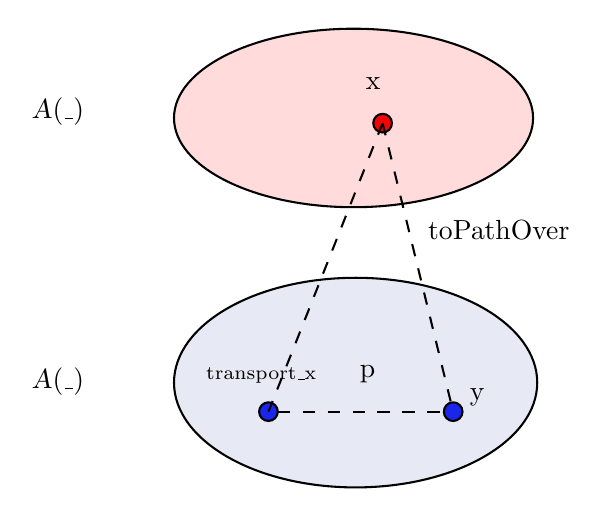
\begin{tikzpicture}[x=0.75pt,y=0.75pt,yscale=-1,xscale=1]
%uncomment if require: \path (0,300); %set diagram left start at 0, and has height of 300

%Shape: Ellipse [id:dp6858943436655307]
\draw  [fill={rgb, 255:red, 231; green, 234; blue, 244 }  ,fill opacity=1 ] (230,230.5) .. controls (230,202.61) and (269.18,180) .. (317.5,180) .. controls (365.82,180) and (405,202.61) .. (405,230.5) .. controls (405,258.39) and (365.82,281) .. (317.5,281) .. controls (269.18,281) and (230,258.39) .. (230,230.5) -- cycle ;
%Shape: Ellipse [id:dp4978096684614166]
\draw  [fill={rgb, 255:red, 255; green, 219; blue, 219 }  ,fill opacity=1 ] (230,103) .. controls (230,79.25) and (268.73,60) .. (316.5,60) .. controls (364.27,60) and (403,79.25) .. (403,103) .. controls (403,126.75) and (364.27,146) .. (316.5,146) .. controls (268.73,146) and (230,126.75) .. (230,103) -- cycle ;
%Shape: Circle [id:dp2462377080592002]
\draw  [fill={rgb, 255:red, 242; green, 5; blue, 5 }  ,fill opacity=1 ] (326,105.5) .. controls (326,103.01) and (328.01,101) .. (330.5,101) .. controls (332.99,101) and (335,103.01) .. (335,105.5) .. controls (335,107.99) and (332.99,110) .. (330.5,110) .. controls (328.01,110) and (326,107.99) .. (326,105.5) -- cycle ;
%Shape: Circle [id:dp1552015327211651]
\draw  [fill={rgb, 255:red, 26; green, 38; blue, 234 }  ,fill opacity=1 ] (360,244.5) .. controls (360,242.01) and (362.01,240) .. (364.5,240) .. controls (366.99,240) and (369,242.01) .. (369,244.5) .. controls (369,246.99) and (366.99,249) .. (364.5,249) .. controls (362.01,249) and (360,246.99) .. (360,244.5) -- cycle ;
%Shape: Circle [id:dp924511868212545]
\draw  [fill={rgb, 255:red, 26; green, 38; blue, 234 }  ,fill opacity=1 ] (271,244.5) .. controls (271,242.01) and (273.01,240) .. (275.5,240) .. controls (277.99,240) and (280,242.01) .. (280,244.5) .. controls (280,246.99) and (277.99,249) .. (275.5,249) .. controls (273.01,249) and (271,246.99) .. (271,244.5) -- cycle ;
%Straight Lines [id:da43777492366231496]
\draw  [dash pattern={on 4.5pt off 4.5pt}]  (280,244.5) -- (360,244.5) ;
%Straight Lines [id:da5251303335065973]
\draw  [dash pattern={on 4.5pt off 4.5pt}]  (330.5,105.5) -- (364.5,244.5) ;
%Straight Lines [id:da2553652396779533]
\draw  [dash pattern={on 4.5pt off 4.5pt}]  (330.5,105.5) -- (275.5,244.5) ;

% Text Node
\draw (321,82) node [anchor=north west][inner sep=0.75pt]   [align=left] {x};
% Text Node
\draw (371,232) node [anchor=north west][inner sep=0.75pt]   [align=left] {y};
% Text Node
\draw (244,222) node [anchor=north west][inner sep=0.75pt]  [font=\scriptsize] [align=left] {transport\_x};
% Text Node
\draw (318,221) node [anchor=north west][inner sep=0.75pt]   [align=left] {p};
% Text Node
\draw (160,92) node [anchor=north west][inner sep=0.75pt]   [align=left] {$\Funapp{\id{A}}{(\earg{\_}{\ileft})}$};
% Text Node
\draw (160,222) node [anchor=north west][inner sep=0.75pt]   [align=left] {$\Funapp{\id{A}}{(\earg{\_}{\iright})}$};
% Text Node
\draw (351,150.92) node [anchor=north west][inner sep=0.75pt]  [rotate=-0.06] [align=left] {toPathOver};

\end{tikzpicture}
\end{center}

The circles represent the two types and points in the circle are elements of the corresponding types. With our definition of equality, we can trivially construct an equality between $\Funapp{\id{A}}{(\earg{\_}{\ileft})}$ and $\Funapp{\id{A}}{(\earg{\_}{\iright})}$. Now, given that the two circles are `equal', intuitively speaking, every point in one circle should have a counterpart in the other circle, and this can be obtained transporting a point along the equality between the two types. The result of transporting $\id{x}$ to the type $\Funapp{\id{A}}{(\earg{\_}{\iright})}$ is a point that we shall call $\id{transport\_x}$. Additionally, suppose also that we have an equality between $\id{transport\_x}$ and $\id{y}$, this is indicated by the path $\id{p}$ between the two points in the diagram. Given that $\id{x}$ is transported to $\id{transport\_x}$, and that $\id{transport\_x}$ is equal to $\id{y}$, we also want to be able to say something about the relationship between $\id{x}$ and $\id{y}$. Since they are not of the same type, all we can do is construct a heterogenous equality between them, and this is precisely what the function $\id{toPathOver}$ seeks to do.

\begin{minted}[escapeinside=@@,mathescape=true]{haskell}
toPathOver : (A : I @$\Rrightarrow$@ Type) @$\Rrightarrow$@ (x : A (_ := i0)) @$\Rightarrow$@ (y : A (_ := i1))
             @$\Rightarrow$@ Eq (Eq_cast (p := Eq_eq (f := A)) (f := id) x) y
             @$\rightarrow$@ Heq x y;
toPathOver = @$\lambda$@ _  A @$\Rrightarrow$@ @$\lambda$@ x y @$\Rightarrow$@ @$\lambda$@ p @$\rightarrow$@
  let
    l : Heq x (Eq_cast (p := Eq_eq (f := A)) (f := id) x);
    l = Heq_eq (t := A)
               (f := @$\lambda$@ i @$\Rrightarrow$@
                     I_transp (A := (@$\lambda$@ j @$\Rrightarrow$@ A (_ := I_meet i j)))
                              (r := I_not i) x);
  in
    Eq_cast
        (x := (Eq_cast (p := Eq_eq (f := A)) (f := id) x))
        (y := y)
        (p := p) (f := @$\lambda$@ y' @$\rightarrow$@ Heq x y') l;
\end{minted}

We construct a heterogenous equality between $\id{x}$ and $\id{transport\_x}$ and we concatenate it with the equality proof between $\id{transport\_x}$ and $\id{y}$ to complete the proof.

\begin{minted}[escapeinside=@@,mathescape=true]{haskell}
elimProp : (A : Type_ ?) @$\Rrightarrow$@ (R : A @$\rightarrow$@ A @$\rightarrow$@ Type)
           @$\Rrightarrow$@ (P : Quotient A R @$\rightarrow$@ Type)
           @$\Rrightarrow$@ (prop : (x : Quotient A R) @$\rightarrow$@ isProp (P x))
           @$\rightarrow$@ (f : (x : A) @$\rightarrow$@ P (Quotient_in x))
           @$\rightarrow$@ (x : Quotient A R) @$\rightarrow$@ P x
elimProp = @$\lambda$@ _ _ _ A R P @$\Rrightarrow$@ @$\lambda$@ prop f @$\rightarrow$@
  Quotient_elim
    (R := R) (P := P) f
    (p := @$\lambda$@ a a' r @$\rightarrow$@
      let
        a=a' : Eq (t := Quotient A R) (Quotient_in a) (Quotient_in a')
        a=a' = Quotient_eq (R := R) (a := a) (a' := a') r
        fa=fa' : Heq (f a) (f a')
        fa=fa' = toPathOver
                    (A := @$\lambda$@ i @$\Rrightarrow$@ P (Eq_uneq (p := a=a') (i := i)))
                    (prop (Quotient_in a')
                          (Eq_cast (p := a=a') (f := P) (f a))
                          (f a'))
      in
        fa=fa')
\end{minted}

$\id{toPathOver}$ does the heavy lifting in this proof by allowing us to leverage $\Funapp{\id{isProp}}{(\Funapp{\id{P}}{\id{x}})}$ to easily produce a proof of $\Funapp{\id{Heq}}{(\Funapp{\id{f}}{\id{a}})}{(\Funapp{\id{f}}{\id{a}'})}$.

\section{Holy Trinity?}
Harper's triangle, check this https://existentialtype.wordpress.com/2011/03/27/the-holy-trinity/.

\subsection{Relationship to Logic/Set Theory}
Mention the typical definition of a quotient set, and what it is usually used for.

\subsection{Relationship to Category Theory}
Say that lots of constructs in type theory have equivalents in cat theory. Mention how a quotient type is a coequaliser of two `parallel' functions and compare this to actual code.


\subsubsection{Coequaliser}

\subsubsection{Initial object of quotient set algebras}

\section{Alternatives that were considered}
\subsection{QITs}
Requires significantly more work to accomplish, but approximately the same expressive power as quotient types (how true is this!?)? Or do we draw the line at ``in practice, it has comparable expressivity''?
The implementation of QITs would negatively impact the modularity of inductive types.

\subsection{Quotient by normalisation}
Explain what this is.

Implementation is rather simple, but it seemed to be less expressive and less convenient.

Further investigation led to proof that such quotients can be represented in the type system as it is (refer to Lemma 6.10.8 in HoTT book). Describe proof that the universal property of quotients is respected by such a construction.

\section{Comparison to QITs}
Quotient inductive types are essentially Higher Inductive Types (HITs) that are set-truncated. This essentially provides us with the full range of expressiveness of HITs without higher-dimensional paths (make sure to define paths in the equality section). Such paths are not typically used in day-to-day programming tasks.

Compare to Quotient Haskell and cite examples of types that are convenient to define with QITs but are `tedious' to express as Quotient types.

\appendix

\section{Equational Reasoning}\label{section:eqreasoning}
Equational reasoning provides us with a neat way of expressing proofs in Typer. With the help of some syntactic sugar, this allows us to build chains of equality proofs by using the transitivity property of equality as shown in Section~\ref{subsubsection:eqtransitivity}. This is something that is implemented in the libraries of most proof assistants, such as Agda, Lean, and Lean. This allows lengthy proofs to remain readable as intermediate steps are documented and are clearly seen.

First, we introduce a helper function that simply invokes the transitivity property of equality proofs. This function carries out a single step of equational reasoning.

\begin{minted}[escapeinside=@@,mathescape=true]{haskell}
step-@$\equiv$@ : (x : ?A) @$\rightarrow$@ (y : ?A) @$\rightarrow$@ (z : ?A) @$\rightarrow$@ Eq x y @$\rightarrow$@ Eq y z @$\rightarrow$@ Eq x z
step-@$\equiv$@ _ p q = Eq_trans p q
\end{minted}

Next, we require a second function to conclude a chain of equational reasoning.

\begin{minted}[escapeinside=@@,mathescape=true]{haskell}
qed : (x : ?A) @$\rightarrow$@ Eq x x
qed x = Eq_refl
\end{minted}

To make it all come together, we wrap the above functions with some syntaxic sugar.

\begin{minted}[escapeinside=@@,mathescape=true]{haskell}
_==<_>==_ = step-@$\equiv$@
_@$\qed$@ = qed
\end{minted}

%% TODO:\ Make \_$\qed$ look nicer
\verb|_==<_>==_| can be seen as a mixfix operator, whereas \_$\qed$ is a postfix operator.

When we write the following

\begin{lstlisting}
  x
  ==< p >==
  y
  ==< ... >==
  .
  .
  .
  ==< ... >==
  z $\qed$
\end{lstlisting}

We require that $\id{p}$ be a proof of equality between $\id{x}$ and $\id{y}$, and this can be chained \latinphrase{ad infinitum}. The expression in its entirety is a proof of equality between $\id{x}$ and $\id{z}$. The usage of this is best illustrated via a simple example:

\begin{minted}[escapeinside=@@,mathescape=true]{haskell}
example : (x : ?A) @$\rightarrow$@ (y : ?A) @$\rightarrow$@ (z : ?A) @$\rightarrow$@ (w : ?A)
          @$\rightarrow$@ (p : Eq x y) @$\rightarrow$@ (q : Eq y z) @$\rightarrow$@ (r : Eq z w) @$\rightarrow$@ Eq x w
example x y z w p q r =
  x ==< p >==
  y ==< q >==
  z ==< r >==
  w @$\qed$@
\end{minted}

For a more involved example, we rewrite the proof of \verb|Integer_*DistR+| that was shown in Section~\ref{subsubsection:int-theorems} by using equational reasoning.

\begin{minted}[escapeinside=@@,mathescape=true]{haskell}
Integer_*DistR+ : (x : Integer) @$\rightarrow$@ (y : Integer) @$\rightarrow$@ (z : Integer)
                  @$\rightarrow$@ Eq (Integer_* x (Integer_+ y z))
                        (Integer_+ (Integer_* x y) (Integer_* x z))
Integer_*DistR+ x y z =
  Integer_* x (Integer_+ y z)
  ==< Integer_*-comm x (Integer_+ y z) >==
  Integer_* (Integer_+ y z) x
  ==< Integer_*DistL+ y z x >==
  Integer_+ (Integer_* y x) (Integer_* z x)
  ==< Eq_cong (flip Integer_+ (Integer_* z x)) (Integer_*-comm y x) >==
  Integer_+ (Integer_* x y) (Integer_* z x)
  ==< Eq_cong (Integer_+ (Integer_* x y)) (Integer_*-comm z x) >==
  Integer_+ (Integer_* x y) (Integer_* x z) @$\qed$@
\end{minted}

TODO:\ Consider adding a discussion on additional macros and tactics that could be added to ease the development of such proofs, e.g.\ it would be nice to have rewrite tactics that Lean has to avoid having to invoke Eq\_cong that often

\end{document}
